%!TEX program = xelatex

\documentclass[UTF8]{ctexart}
\usepackage{ctex}

\CTEXsetup[format={\Large\bfseries}]{section}

\usepackage[version=3]{mhchem} % Package for chemical equation typesetting
\usepackage{siunitx} % Provides the \SI{}{} and \si{} command for typesetting SI units
\usepackage{graphicx} % Required for the inclusion of images
% \graphicspath{{assets/}}
\usepackage{natbib} % Required to change bibliography style to APA
\usepackage{amsmath} % Required for some math elements 
\usepackage{amssymb}
\usepackage[hidelinks]{hyperref}
\usepackage{makecell} % 3 Packages for flexible tabular
\usepackage{multirow}
\usepackage{multicol}

\usepackage{pdfpages}  % include pdf pages for original data etc.

\usepackage{geometry}% 版面大小
\geometry{a4paper,scale=0.7}

\usepackage{fontspec}

\setCJKfamilyfont{hwxk}{STXingkai}% 字体
\newcommand{\hwxk}{\CJKfamily{hwxk}}

\usepackage{fancyhdr}% 页眉页脚
\fancypagestyle{EE_Digital1Exp_template}{
    \fancyhead[L]{\Large {\hwxk 南京大学电子科学与工程学院}}
    \fancyhead[R]{数字系统1实验报告}
    \fancyfoot[c]{- \thepage \ -}
    \renewcommand\footrulewidth{0pt}
}

% 4级目录
\setcounter{secnumdepth}{4}
\setcounter{tocdepth}{4}

\usepackage{graphicx} % Packages for figures
\usepackage{caption2}
\usepackage{subfigure}
\usepackage{float}

\usepackage{listings} % Packages for code block
\usepackage{xcolor}

% for verilog code coloring
\definecolor{vgreen}{RGB}{104,180,104}
\definecolor{vblue}{RGB}{49,49,255}
\definecolor{vorange}{RGB}{255,143,102}

\lstdefinestyle{verilog-style}
{
    language=Verilog,
    basicstyle=\small\ttfamily,
    keywordstyle=\color{vblue},
    identifierstyle=\color{black},
    commentstyle=\color{vgreen},
    numbers=left,
    numberstyle=\tiny\color{black},
    numbersep=10pt,
    tabsize=8,
    moredelim=*[s][\colorIndex]{[}{]},
    literate=*{:}{:}1
}

\makeatletter
\newcommand*\@lbracket{[}
\newcommand*\@rbracket{]}
\newcommand*\@colon{:}
\newcommand*\colorIndex{%
    \edef\@temp{\the\lst@token}%
    \ifx\@temp\@lbracket \color{black}%
    \else\ifx\@temp\@rbracket \color{black}%
    \else\ifx\@temp\@colon \color{black}%
    \else \color{vorange}%
    \fi\fi\fi
}
\makeatother

\usepackage{trace}




%设置图片、表格编号
\renewcommand{\thetable}{\thesubsection{}-\arabic{table}}
\renewcommand{\thefigure}{\thesubsection{}-\arabic{figure}}
\renewcommand{\thefigure}{\thesubsection{}-\arabic{equation}}
\usepackage{amsmath}
\numberwithin{figure}{subsection}
\numberwithin{table}{subsection}
\numberwithin{equation}{subsection}

\setlength\parindent{6pt} % Removes all indentation from paragraphs

\renewcommand{\labelenumi}{\alph{enumi}.} % Make numbering in the enumerate environment by letter rather than number (e.g. section 6)

%\usepackage{times} % Uncomment to use the Times New Roman font

%----------------------------------------------------------------------------------------
%	DOCUMENT INFORMATION
%----------------------------------------------------------------------------------------

\title{\textbf{实验三\ 移位寄存器}} % Title

\author{电子科学与工程学院\ 刘时宜\ 201180078} % Author name

\date{} % Date for the report

\begin{document}

\pagestyle{EE_Digital1Exp_template}

\maketitle % Insert the title, author and date

\begin{center}
    \begin{tabular}{l r}
    实验日期: & 2021年11月17日 \\ % Date the experiment was performed
     & 2021年11月24日 \\ % Date the experiment was performed
    指导老师: & 高健 % Instructor/supervisor
    \end{tabular}
    \par 点击目录、书签栏、以及行文中的图表标号的均可跳转至相应页面
    \end{center}
    
% If you wish to include an abstract, uncomment the lines below
% \begin{abstract}
% Abstract text
% \end{abstract}

\tableofcontents

\section{实验目的}
\begin{enumerate}
    \item 验证移位寄存器的功能
    \item 利用移位寄存器搭建数据收发器
\end{enumerate}

\section{实验仪器与主要器材}
\begin{center}
    \begin{tabular}{ll}
        \textbf{仪器:} & \\
        Basys3 FPGA 开发板 & 1台\\
        KEYSIGHT DSOX1102AG 示波器 & 1台\\
        示波器高频探头 & 1套\\
        ROGOL DM3068 万用表 & 1台\\
        \textbf{软件:} & \\
        Multisim & 14.1 \\
        Digilent Adept & 2.19.2 \\
        Vivado & 2015.4 \\
        \textbf{耗材:} & \\
        导线 & 若干 \\
    \end{tabular}
\end{center}

\section{实验原理}
\par 在各种复杂的数字电路中,不但需要对二值信号进行算术运算和逻辑运算,还经常需要将这些信号和运算结果保存下来。因此,需要使用具有记忆功能的基本逻辑单元。能够储存1位二值信号的基本单元电路统称触发器。
\par 寄存器用于储存一组二值代码,它被广泛运用于各类数字系统和数字计算机当中。因为一个触发器能够储存1位二值数据,所以用N个触发器组成的寄存器可以储存N位二进制代码。
\par 移位寄存器除了具有储存代码的功能以外,还具有移位功能。所谓移位功能,是指寄存器里储存的代码能够在移位脉冲的作用下依次左移或者右移。因此,移位寄存器不但可以用来寄存代码,还可以用来实现数据的串行-并行转换、数值的运算以及数据处理等。

\section{实验过程}
\subsection{移位寄存器单源周期触发测试}
\par 实验电路如图\ref{single source citcuit}所示。将已经编译好的bit文件下载到开发板上,观察实验现象。

\begin{figure}[H]
    \begin{center}
        \includegraphics[width=0.8\textwidth]{pics/1S-V2/circuit.jpg}
    \end{center}
    \caption{移位寄存器单源周期触发测试电路}
    \label{single source citcuit}
\end{figure}

\subsubsection{实验结果}
使用示波器测量引脚JB0与JB2的波形图\ref{1S-V2 osci}所示:
\begin{figure}[H]
    \centering
    \subfigure[SW1]{
    \includegraphics[width=0.45\textwidth]{pics/1S-V2/1.jpg}}
    \subfigure[SW2]{
    \includegraphics[width=0.45\textwidth]{pics/1S-V2/2.jpg}}
    \subfigure[SW3]{
    \includegraphics[width=0.45\textwidth]{pics/1S-V2/3.jpg}}
    \subfigure[SW4]{
    \includegraphics[width=0.45\textwidth]{pics/1S-V2/4.jpg}}
    \subfigure[SW2、SW6]{
    \includegraphics[width=0.45\textwidth]{pics/1S-V2/26.jpg}}
    \subfigure[SW0、SW2、SW6]{
    \includegraphics[width=0.45\textwidth]{pics/1S-V2/026.jpg}}
    \subfigure[SW7、SW8]{
    \includegraphics[width=0.45\textwidth]{pics/1S-V2/78.jpg}}
    \caption{移位寄存器单源周期触发测试-输出波形}
    \label{1S-V2 osci}
\end{figure}
可以看到在图(a)~(d)中,随着开关位置的变化,移位寄存器最高位的输出波形(通道2,绿色)随之相较移位寄存器置数信号位置依次向后移动,反映了移位寄存器数据移位的功能特点。在多输入时,可以看到移位寄存器将并行输入转换成为了串行输出。图(g)中的输入数据为我的学号。

\par 切换时钟频率到秒分频,观察LED灯光情况,测试视频已随邮件附件发送,分别为“1s-1.mp4”,“1s-2.mp4”。


\subsection{移位寄存器单次触发测试电路}
自己搭建实验电路图如图\ref{S-V2}所示。电路搭建完成后,生成bit文件并下载至开发板上,验证试验现象。

\begin{figure}[H]
    \begin{center}
        \includegraphics[width=0.8\textwidth]{pics/S-V2/circuit.png}
    \end{center}
    \caption{移位寄存器单次触发测试电路}
    \label{S-V2}
\end{figure}

测试引脚JB2(通道1,绿色)、JB0(通道1,黄色)的波形如图\ref{S-V2 chaos}所示。可以看到,无移位输入信号时,JB0的波形混乱,怀疑为电路工作频率过高所致电路行为不正常,因此更改分频电路模块,降低电路工作频率,更改的分频电路模块如图\ref{S-V2 mod freq}所示,更改的部分用浅蓝色连线标明。

\begin{figure}[H]
    \begin{center}
        \includegraphics[width=0.8\textwidth]{pics/S-V2/circuit.png}
    \end{center}
    \caption{原电路实验波形}
    \label{S-V2 chaos}
\end{figure}


\begin{figure}[H]
    \begin{center}
        \includegraphics[width=0.8\textwidth]{pics/S-V2/MODIFY FREQ DIV.png}
    \end{center}
    \caption{分频电路更改}
    \label{S-V2 mod freq}
\end{figure}

更改后电路波形正常,为验证JK触发器在不同J、K输入条件下的置数情况,调整J、K的输入值,测试JB2(通道1,绿色)、JB0(通道1,黄色)的波形如图\ref{S-V2 osci}所示。

\begin{figure}[H]
    \centering
    \subfigure[J = 0, K = 0, 保持置数0]{
    \includegraphics[width=0.45\textwidth]{pics/S-V2/j0k00.jpg}}
    \subfigure[J = 0, K = 0, 保持置数1]{
    \includegraphics[width=0.45\textwidth]{pics/S-V2/j0k01.jpg}}
    \subfigure[J = 0, K = 1]{
    \includegraphics[width=0.45\textwidth]{pics/S-V2/j0k1.jpg}}
    \subfigure[J = 1, K = 0]{
    \includegraphics[width=0.45\textwidth]{pics/S-V2/j1k0.jpg}}
    \subfigure[J = 1, K = 1]{
    \includegraphics[width=0.45\textwidth]{pics/S-V2/j1k1.jpg}}
    
    \caption{移位寄存器单次触发测试电路-输出波形}
    \label{S-V2 osci}
\end{figure}

可以看到,J = 0, K = 0 时,触发器次态与现态相同,JK触发器工作在保持状态;J = 0, K = 1时,触发器次态为0,为置零工作模式;J = 1, K = 0时,触发器次态为1,为置一工作模式;J = 1, K = 1时,触发器次态与现态相反,触发器在0、1之间不停翻转。总而言之,通过实验验证了JK触发器在不同输入状态下的工作情况,与理论相符。

\par 切换时钟频率到秒分频,观察LED灯光情况,测试视频已随邮件附件发送,为“s-1.mp4”。

\subsection{数据收发器}
利用移位寄存器构成数据收发器,电路原型如图\ref{DataSR circuit prototype}所示。
\par 其中发送端利用计数器结合按键时间,产生随机数,随后送到触发器中进行显示,并连接到并入串出移位寄存器,待发送信号后将数据发出。发送数据的第一位恒为高电平,用于触发接收端读取报文数据并进行处理显示。
\par 接收端接受5位数据,其中第一位为数据报头,用于触发数据接收过程。当串入并出移位寄存器第5为位高电平时,D锁存器被使能,读取低4位数据信息,并在移位寄存器清零后保存数据信息,送至下级电路进行数据显示。

\begin{figure}[H]
    \centering
    \subfigure[数据发送端]{
    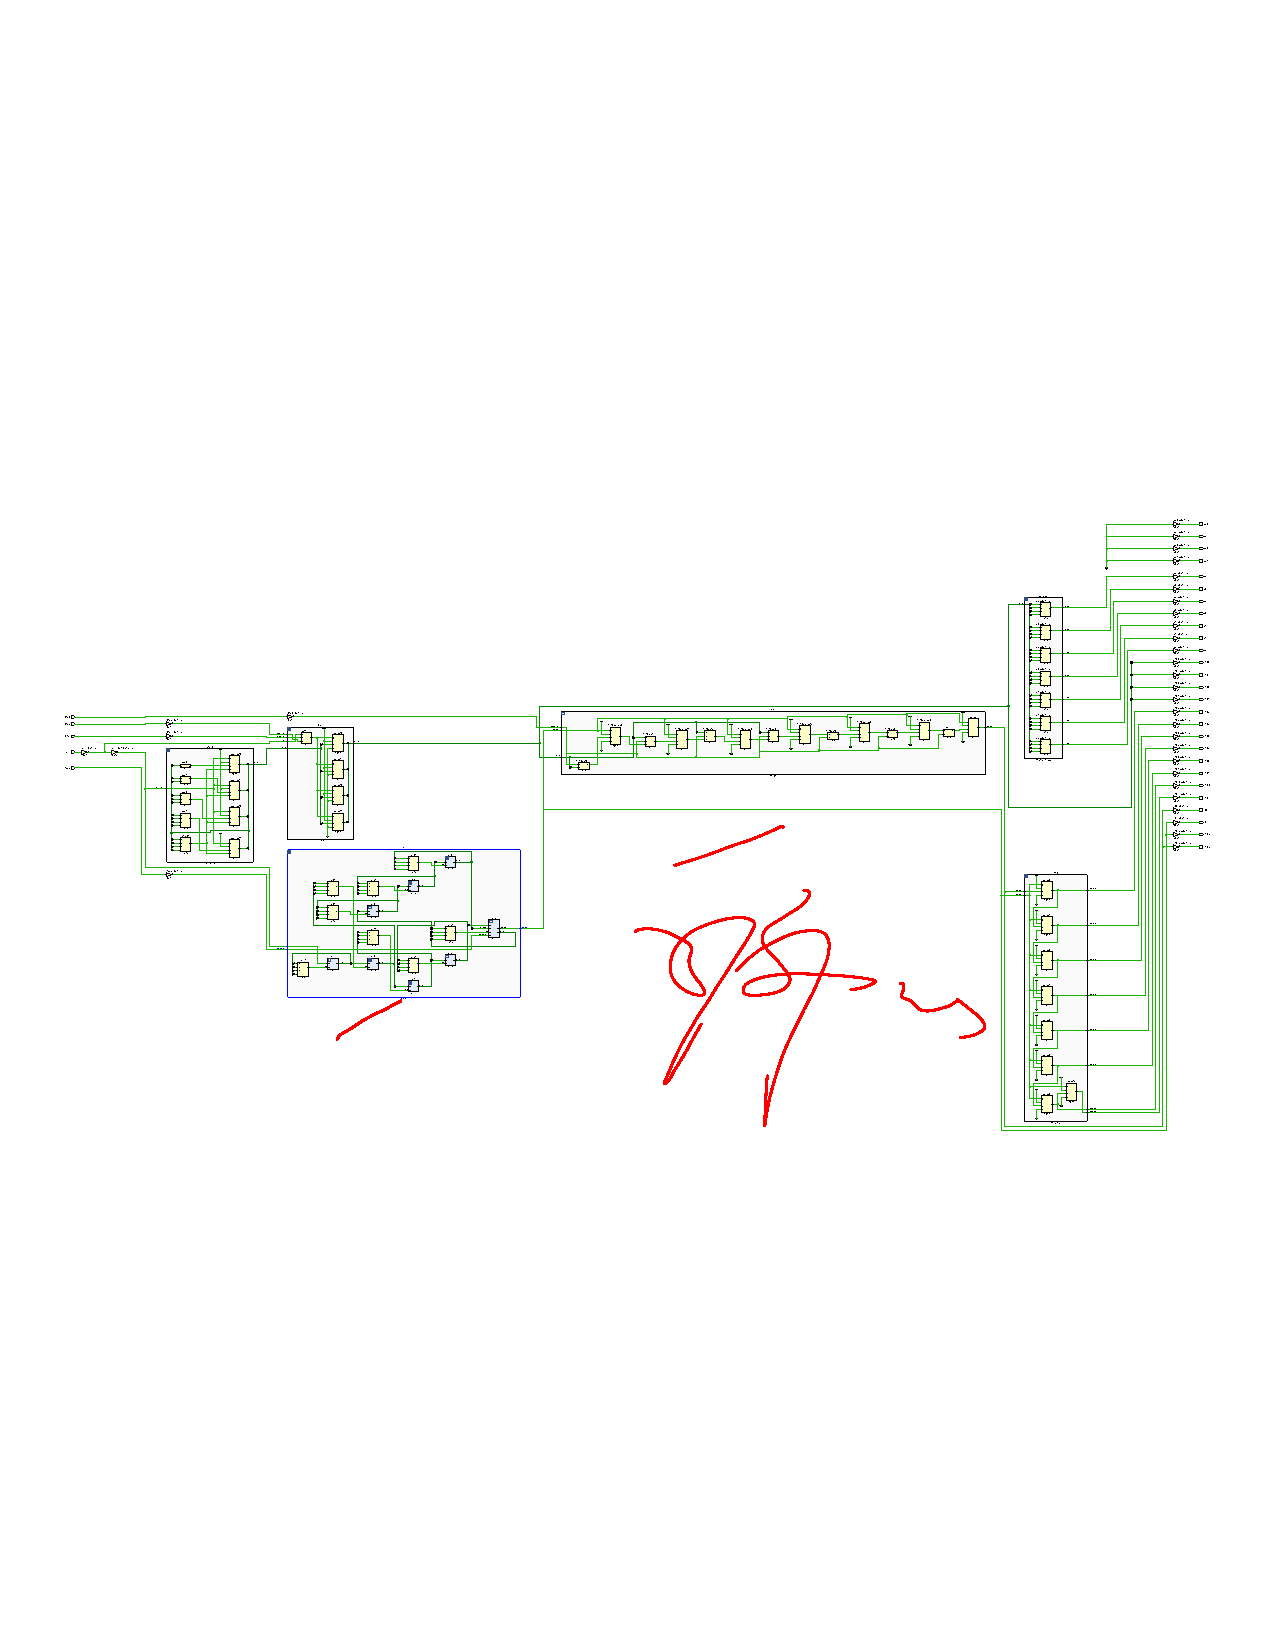
\includegraphics[width=0.45\textwidth]{pics/DataSR/sender.jpg}}
    \subfigure[数据接收端]{
    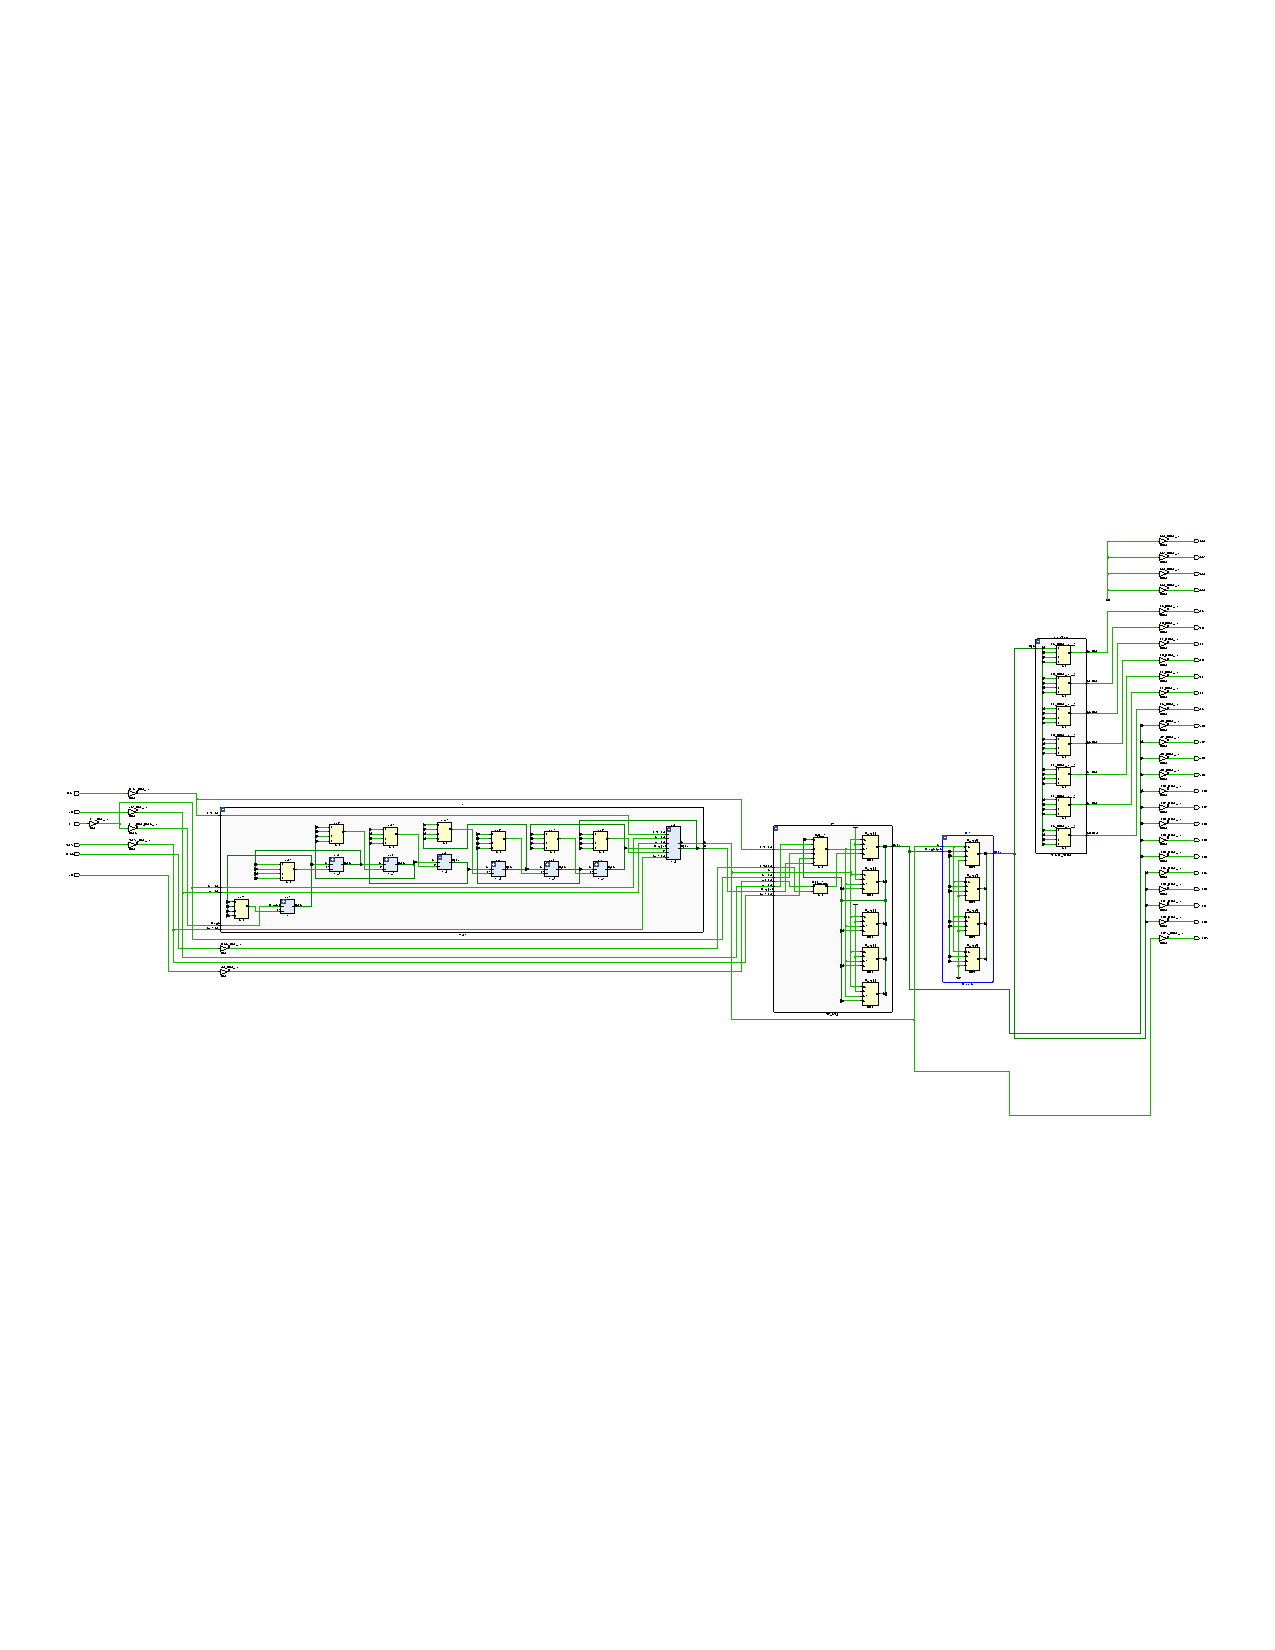
\includegraphics[width=0.45\textwidth]{pics/DataSR/receiver.jpg}}
    \caption{数据收发器-原型电路}
    \label{DataSR circuit prototype}
\end{figure}


\subsubsection{数据发送端电路搭建}
\par {\color{red}\textbf{以下所有电路搭建过程均由verilog + Vivado进行实现。}}
\par 首先,电路所需的各个模块:
\paragraph{十分频模块}
\begin{lstlisting}[style={verilog-style}]
module ten(
    input clock,
    output ten
    );
    reg [3:0]Q;
    always @(posedge clock) begin
        if (Q <= 8) begin
            Q = Q + 1;
        end
        else
            Q = 0;
    end
    assign ten = Q[3];
endmodule
\end{lstlisting}

\paragraph{分频电路模块}~
\par 利用刚才搭建的十分频模块进行级联,即可得到不同频率的时钟信号,将所有得到的信号送至输出端口CP,以备后级电路使用。
\begin{lstlisting}[style={verilog-style}]
module freq_div(
    input clock,
    output [10:1]CP
    );

    ten div1(clock, CP[1]);
    ten div2(CP[1], CP[2]);
    ten div3(CP[2], CP[3]);
    ten div4(CP[3], CP[4]);
    ten div5(CP[4], CP[5]);
    ten div6(CP[5], CP[6]);
    ten div7(CP[6], CP[7]);
    ten div8(CP[7], CP[8]);
    ten div9(CP[8], CP[9]);
    ten div10(CP[9], CP[10]);
    
endmodule
\end{lstlisting}

\paragraph{数据选择器}~
\par 用于选择时钟频率,使电路工作在不同频率下。
\begin{lstlisting}[style={verilog-style}]
module mux2to1(
    input s,
    input [1:0] data,
    output reg out
    );
    always @(data or s) begin
        out = s ? data[1]:data[0];
    end
endmodule
\end{lstlisting}

\paragraph{十进制计数器}~
\par 用于配合时钟信号,产生随机数。
\begin{lstlisting}[style={verilog-style}]
module counter10(
    input clk,
    input reset,
    output [3:0] Q
    );
    reg [3:0]number;
    always @(posedge clk or posedge reset) begin
        if (reset) begin
            number = 0;
        end
        else if(number < 9) begin
            number = number+1;
        end
        else
            number = 0;
    end
    assign Q = number;
endmodule
\end{lstlisting}

\paragraph{4位D触发器}~
\par 用于配合十进制计数器,保存计数器产生的随机数准备发送。
\begin{lstlisting}[style={verilog-style}]
module FF_D4(
    input clk,
    input [3:0] D,
    output [3:0] Q
    );
    reg [3:0]W;
    always @(posedge clk) begin
        W = D;
    end
    assign Q = W;
endmodule
\end{lstlisting}

\paragraph{4位D触发器}~
\par 用于配合十进制计数器,保存计数器产生的随机数准备发送。
\begin{lstlisting}[style={verilog-style}]
module FF_D4(
    input clk,
    input [3:0] D,
    output [3:0] Q
    );
    reg [3:0]W;
    always @(posedge clk) begin
        W = D;
    end
    assign Q = W;
endmodule
\end{lstlisting}

\paragraph{8位并入串出移位寄存器}~
\par 用于D触发器,在数据发送信号到来时进行数据发送。
\begin{lstlisting}[style={verilog-style}]
module SR_8P(
    input [7:0] DataIn,
    input clk,
    inout load,
    output reg Q
    );

    reg [7:0]ShiftData;
    always @(posedge clk) begin
        if (load) begin
            ShiftData <= DataIn;
            Q <= ShiftData[7];
        end
        else begin
            ShiftData <= {ShiftData[6:0],1'b0};
            Q <= ShiftData[7];
        end
    end
endmodule
\end{lstlisting}

\paragraph{8位串入并移位寄存器}~
\par 连接8位并入串出移位寄存器输出端,并将并行输出连接至LED进行显示,便于观察电路工作状态。
\begin{lstlisting}[style={verilog-style}]
module SR_NS_C(Data, clk, clr, Q);
    parameter n = 8;
    input Data;
    input clk, clr;
    output reg [n-1:0] Q;

    always @(posedge clk) begin
        if(clr)
            Q = 0;
        else
            Q = {Q[n-2:0], Data};
    end
endmodule
\end{lstlisting}

\paragraph{静态显示模块}~
\par 由BCD-数码管译码器以及相应数码管连接电路构成,用于将输入数据显示到数码管上。
\begin{lstlisting}[style={verilog-style}]
module BCD_dec(
    input [3:0]D,
    output reg [6:0]Q
    );

    always @(D) begin
        case(D)
            0: Q = {1'b1, 1'b1, 1'b1, 1'b1, 1'b1, 1'b1, 1'b0};
            1: Q = {1'b0, 1'b1, 1'b1, 1'b0, 1'b0, 1'b0, 1'b0};
            2: Q = {1'b1, 1'b1, 1'b0, 1'b1, 1'b1, 1'b0, 1'b1};
            3: Q = {1'b1, 1'b1, 1'b1, 1'b1, 1'b0, 1'b0, 1'b1};
            4: Q = {1'b0, 1'b1, 1'b1, 1'b0, 1'b0, 1'b1, 1'b1};
            5: Q = {1'b1, 1'b0, 1'b1, 1'b1, 1'b0, 1'b1, 1'b1};
            6: Q = {1'b1, 1'b0, 1'b1, 1'b1, 1'b1, 1'b1, 1'b1};
            7: Q = {1'b1, 1'b1, 1'b1, 1'b0, 1'b0, 1'b0, 1'b0};
            8: Q = {1'b1, 1'b1, 1'b1, 1'b1, 1'b1, 1'b1, 1'b1};
            9: Q = {1'b1, 1'b1, 1'b1, 1'b1, 1'b0, 1'b1, 1'b1};
            default : Q = 0;
        endcase
    end
endmodule

module STATIC_SHOW (
    input [3:0]D,
    output [6:0]LED_digit,
    output [3:0]enable
);

    wire [6:0]BCDcode;
    assign enable = 0;
    
    BCD_dec BCDdec(D, BCDcode);
    assign LED_digit = ~BCDcode;

endmodule
\end{lstlisting}

\paragraph{主电路模块}~
\par 将刚才构建的各个电路模块进行级联,构成完整的数据发送端电路。
\begin{lstlisting}[style={verilog-style}]
module main(
    input BTND, BTNL, BTNC,
    input CLK,
    input SW15,
    output LED0, LED1, LED2, LED3, LED15,  
    output LED14, //clkUsed
    output LED4, LED5, LED6, LED7,LED8, LED9, LED10, LED11, //for testing
    output JB0,JB1,
    output CA, CB, CC, CD, CE, CF, CG, AN3, AN2, AN1, AN0
    );
    
    wire [3:0]CTN10out;
    wire triggerData;
    wire [3:0]data; // def MSB on the left hand side!!!

    // getting data to be transmitted
    assign triggerData = (BTNL && CLK) || BTNC;
    counter10 CTN10(CLK, 1'b0, CTN10out);
    FF_D4 D4_1(triggerData, CTN10out, data);

    //showing data
    assign {LED3,LED2,LED1,LED0} = data;
    STATIC_SHOW sta_show1(data,{CA, CB, CC, CD, CE, CF, CG}, {AN3, AN2, AN1, AN0});

    //getting low freq clk signal
    wire [10:1]clkAll;
    wire [1:0]clkOpt;
    wire clkUsed;
    freq_div f1(CLK, clkAll);
    assign clkOpt = {clkAll[5], clkAll[8]};
    mux2to1 M1(SW15, clkOpt,clkUsed);
    assign JB1 = clkUsed;
    assign LED14 = clkUsed;

    //transmitting data
    wire sendOut;
    SR_8P SR1({1'b0, 1'b1, data, 1'b0, 1'b0}, clkUsed, BTND, sendOut);
    assign JB0 = sendOut;
    assign LED15 = sendOut;

    // for testing
    SR_NS_C SR2(sendOut, clkUsed, 1'b0, {LED11, LED10, LED9, LED8,LED7, LED6, LED5, LED4});

endmodule
\end{lstlisting}


\subsubsection{数据接收端电路搭建}
\par 数据接收端的电路原型存在问题,详细叙述如下:
\par 原型电路中,接收端电路D锁存器使能端与移位寄存器输出第5位相连,为异步工作模式。当移位寄存器清零时,第5位与第4位“同时”清零,“同时”,D锁存器使能端归零,D锁存器不再接受数据。
\par 然而,实际电路中存在信号传播时间问题,移位寄存器输出置零顺序存在竞争。由Vivade综合出的电路\textbf{移位寄存器输出第5位晚于低4位置零,使得D锁存器在移位寄存器归零后仍然读取并保存数据,使得正常数据无法保存,稳定时D锁存器存储数字为'0000'}。
\par 为解决信号传播时间问题,将D锁存器的使能端由异步工作模式更换为同步工作模式,引入时钟信号,使得锁存器在数据清零前停止读取数据,解决这个问题。
\begin{figure}[H]
    \begin{center}
        \includegraphics[width=0.8\textwidth]{pics/DataSR/receiver problem.png}
    \end{center}
    \caption{接收端电路问题}
    \label{receiver problem}
\end{figure}

\par 此外,更改了原型电路,将数据显示模块改为动态显示模块,使得数码管4位可以显示4个不同的数字。同时搭建16位移位寄存器,存储4位10进制数所需的16位BCD码。在有数据到来时,以4位为整体进行移位,达到显示移位的效果。


\paragraph{分频电路模块}~
\par 数据接收端本身不需要此模块,引入此模块用于单板测试之用。
\begin{lstlisting}[style={verilog-style}]
module ten(
    input clock,
    output ten
    );
    reg [3:0]Q;
    always @(posedge clock) begin
        if (Q <= 8) begin
            Q = Q + 1;
        end
        else
            Q = 0;
    end
    assign ten = Q[3];
endmodule

module freq_div(
    input clock,
    output [10:1]CP
    );

    ten div1(clock, CP[1]);
    ten div2(CP[1], CP[2]);
    ten div3(CP[2], CP[3]);
    ten div4(CP[3], CP[4]);
    ten div5(CP[4], CP[5]);
    ten div6(CP[5], CP[6]);
    ten div7(CP[6], CP[7]);
    ten div8(CP[7], CP[8]);
    ten div9(CP[8], CP[9]);
    ten div10(CP[9], CP[10]);
    
endmodule
\end{lstlisting}

\paragraph{分频电路模块}~
\par 数据接收端本身不需要此模块,引入此模块用于单板测试之用。
\begin{lstlisting}[style={verilog-style}]
module ten(
    input clock,
    output ten
    );
    reg [3:0]Q;
    always @(posedge clock) begin
        if (Q <= 8) begin
            Q = Q + 1;
        end
        else
            Q = 0;
    end
    assign ten = Q[3];
endmodule

module freq_div(
    input clock,
    output [10:1]CP
    );

    ten div1(clock, CP[1]);
    ten div2(CP[1], CP[2]);
    ten div3(CP[2], CP[3]);
    ten div4(CP[3], CP[4]);
    ten div5(CP[4], CP[5]);
    ten div6(CP[5], CP[6]);
    ten div7(CP[6], CP[7]);
    ten div8(CP[7], CP[8]);
    ten div9(CP[8], CP[9]);
    ten div10(CP[9], CP[10]);
    
endmodule

module mux2to1( // 用于选择时钟信号来源
    input s,
    input [1:0] data,
    output reg out
    );
    always @(data or s) begin
        out = s ? data[1]:data[0];
    end
endmodule
\end{lstlisting}

\paragraph{8位串入并出移位寄存器}~
\par 用于接收数据发送端送来的数据
\begin{lstlisting}[style={verilog-style}]
module SR_NS_C(Data, clk, clr, Q);
    parameter n = 8;
    input Data;
    input clk, clr;
    output reg [n-1:0] Q;

    always @(posedge clk or posedge clr) begin
        if (clr) begin
            Q <= 0;
        end
        else
            Q <= {Q[n-2:0], Data};
    end

endmodule
\end{lstlisting}

\paragraph{8位串入并出移位寄存器}~
\par 用于接收数据发送端送来的数据。
\begin{lstlisting}[style={verilog-style}]
module SR_NS_C(Data, clk, clr, Q);
    parameter n = 8;
    input Data;
    input clk, clr;
    output reg [n-1:0] Q;

    always @(posedge clk or posedge clr) begin
        if (clr) begin
            Q <= 0;
        end
        else
            Q <= {Q[n-2:0], Data};
    end

endmodule
\end{lstlisting}

\paragraph{D锁存器}~
\par 用于检测数据到达情况并读取、保存到达的数据。
\par 注意,为了解决上文所述的信号竞争问题,引入了时钟信号,做同步使能。
\begin{lstlisting}[style={verilog-style}]
module DLatchN(Data, set, clk, Q);
    parameter n = 4;
    input [n-1:0]Data;
    input set,clk;
    output reg [n-1:0]Q;

    always @(negedge clk) begin
        if (set) begin
            Q = Data;
        end
    end
endmodule
\end{lstlisting}


\paragraph{16位BCD码移位寄存器}~
\par 用于保存4位十进制数,送至动态显示模块进行输出。
\begin{lstlisting}[style={verilog-style}]
module SR_16_4BIT_BLOCK(
    input   wire    [3:0]   data,
    input   wire            en,
    input                   clk,
    output  reg     [15:0]  Q
    );

    always @(negedge clk) begin
        if(en)
            Q = {Q[11:0], data};
    end
endmodule
\end{lstlisting}

\paragraph{动态显示模块}~
\par 用于显示4位不相同的十进制数。
\begin{lstlisting}[style={verilog-style}]
module dyn_show(
    input   wire    [15:0]  Data,
    input   wire            clk,
    output  wire    [6:0]   LED,
    output  reg     [3:0]   LED_en
    );

    reg     [1:0]   state;
    reg     [3:0]   selected;

    BCD_dec BCD(selected, LED);

    always @(posedge clk)begin
        case (state)
            0: {selected,LED_en} <= {Data[3:0]   ,4'b1110};
            1: {selected,LED_en} <= {Data[7:4]   ,4'b1101};
            2: {selected,LED_en} <= {Data[11:8]  ,4'b1011};
            3: {selected,LED_en} <= {Data[15:12] ,4'b0111};
        endcase
        state <= state+1;
    end
endmodule

module BCD_dec(
    input [3:0]D,
    output reg [6:0]Q
    );

    always @(D) begin
        case(D)
            0: Q = {1'b1, 1'b1, 1'b1, 1'b1, 1'b1, 1'b1, 1'b0};
            1: Q = {1'b0, 1'b1, 1'b1, 1'b0, 1'b0, 1'b0, 1'b0};
            2: Q = {1'b1, 1'b1, 1'b0, 1'b1, 1'b1, 1'b0, 1'b1};
            3: Q = {1'b1, 1'b1, 1'b1, 1'b1, 1'b0, 1'b0, 1'b1};
            4: Q = {1'b0, 1'b1, 1'b1, 1'b0, 1'b0, 1'b1, 1'b1};
            5: Q = {1'b1, 1'b0, 1'b1, 1'b1, 1'b0, 1'b1, 1'b1};
            6: Q = {1'b1, 1'b0, 1'b1, 1'b1, 1'b1, 1'b1, 1'b1};
            7: Q = {1'b1, 1'b1, 1'b1, 1'b0, 1'b0, 1'b0, 1'b0};
            8: Q = {1'b1, 1'b1, 1'b1, 1'b1, 1'b1, 1'b1, 1'b1};
            9: Q = {1'b1, 1'b1, 1'b1, 1'b1, 1'b0, 1'b1, 1'b1};
            default : Q = 0;
        endcase
    end
endmodule
\end{lstlisting}

\paragraph{主电路模块}~
\par 连接以上各模块,形成完整的接收端电路。
\begin{lstlisting}[style={verilog-style}]
module main(
    input JA0, // sender data input
    input BTNL,BTNU,//BTNU for testing
    input CLK,
    input JA1,
    input SW15, // for selecting clk signal for testing

    output CA,CB,CC,CD,CE,CF,CG,AN0,AN1,AN2,AN3,
    output JB0, JB1, JB2, JB3,
    output LED4, LED3, LED2, LED1, LED0, // for SR1out[3:0]
    output LED8, LED7, LED6, LED5, //for DL1out
    output LED15 // for watching clk signal
    );

    parameter nbit = 8;

    //getiing clk signal
    wire psuedoCLK;
    assign psuedoCLK = (BTNL && CLK) || JA1;
    wire [10:1]clkAll;
    wire clkOpt;
    wire clkUsed;
    freq_div f1(CLK, clkAll);
    assign clkOpt = clkAll[8];
    mux2to1 M1(SW15, {clkOpt, psuedoCLK} ,clkUsed);
    assign LED15 = clkUsed;


    // get signal and trigger storage
    // SR1out[4] is for triggering data storage and reset, SR1out[3:0] is valid data signal.
    wire SR1clr;
    wire [nbit-1:0]SR1out;
    wire dataIn;
    assign dataIn = JA0 || BTNU;
    SR_NS_C #(.n(nbit))R1(dataIn, psuedoCLK, SR1clr ,SR1out);
    
    assign SR1clr = SR1out[4] && (~clkUsed);
    assign {JB3, JB2, JB1, JB0} = SR1out[3:0];
    assign {LED4, LED3, LED2, LED1, LED0} = SR1out[4:0];

    //storing data
    wire [3:0]DL1out;
    DLatchN #(.n(4))DL1(SR1out[3:0], SR1out[4], clkUsed, DL1out);

    // dyn show data

    wire    [15:0]  dynLED;
    SR_16_4BIT_BLOCK SR_dyn_out(DL1out, SR1out[4], clkUsed, dynLED);
    dyn_show dyn(dynLED, clkAll[3], {CA,CB,CC,CD,CE,CF,CG}, {AN3, AN2, AN1, AN0});



    //showing data
    //STATIC_SHOW staticShow(DL1out, {CA,CB,CC,CD,CE,CF,CG}, {AN0,AN1,AN2,AN3});
    //assign {LED8, LED7, LED6, LED5} = DL1out;


endmodule
\end{lstlisting}


\subsubsection{综合、编译、下载至开发板进行实验}
\par 综合出的发送端、接收端实验电路如图\ref{send synth circuit}、图\ref{receiver synth circuit}所示。

\begin{figure}[H]
    \begin{center}
        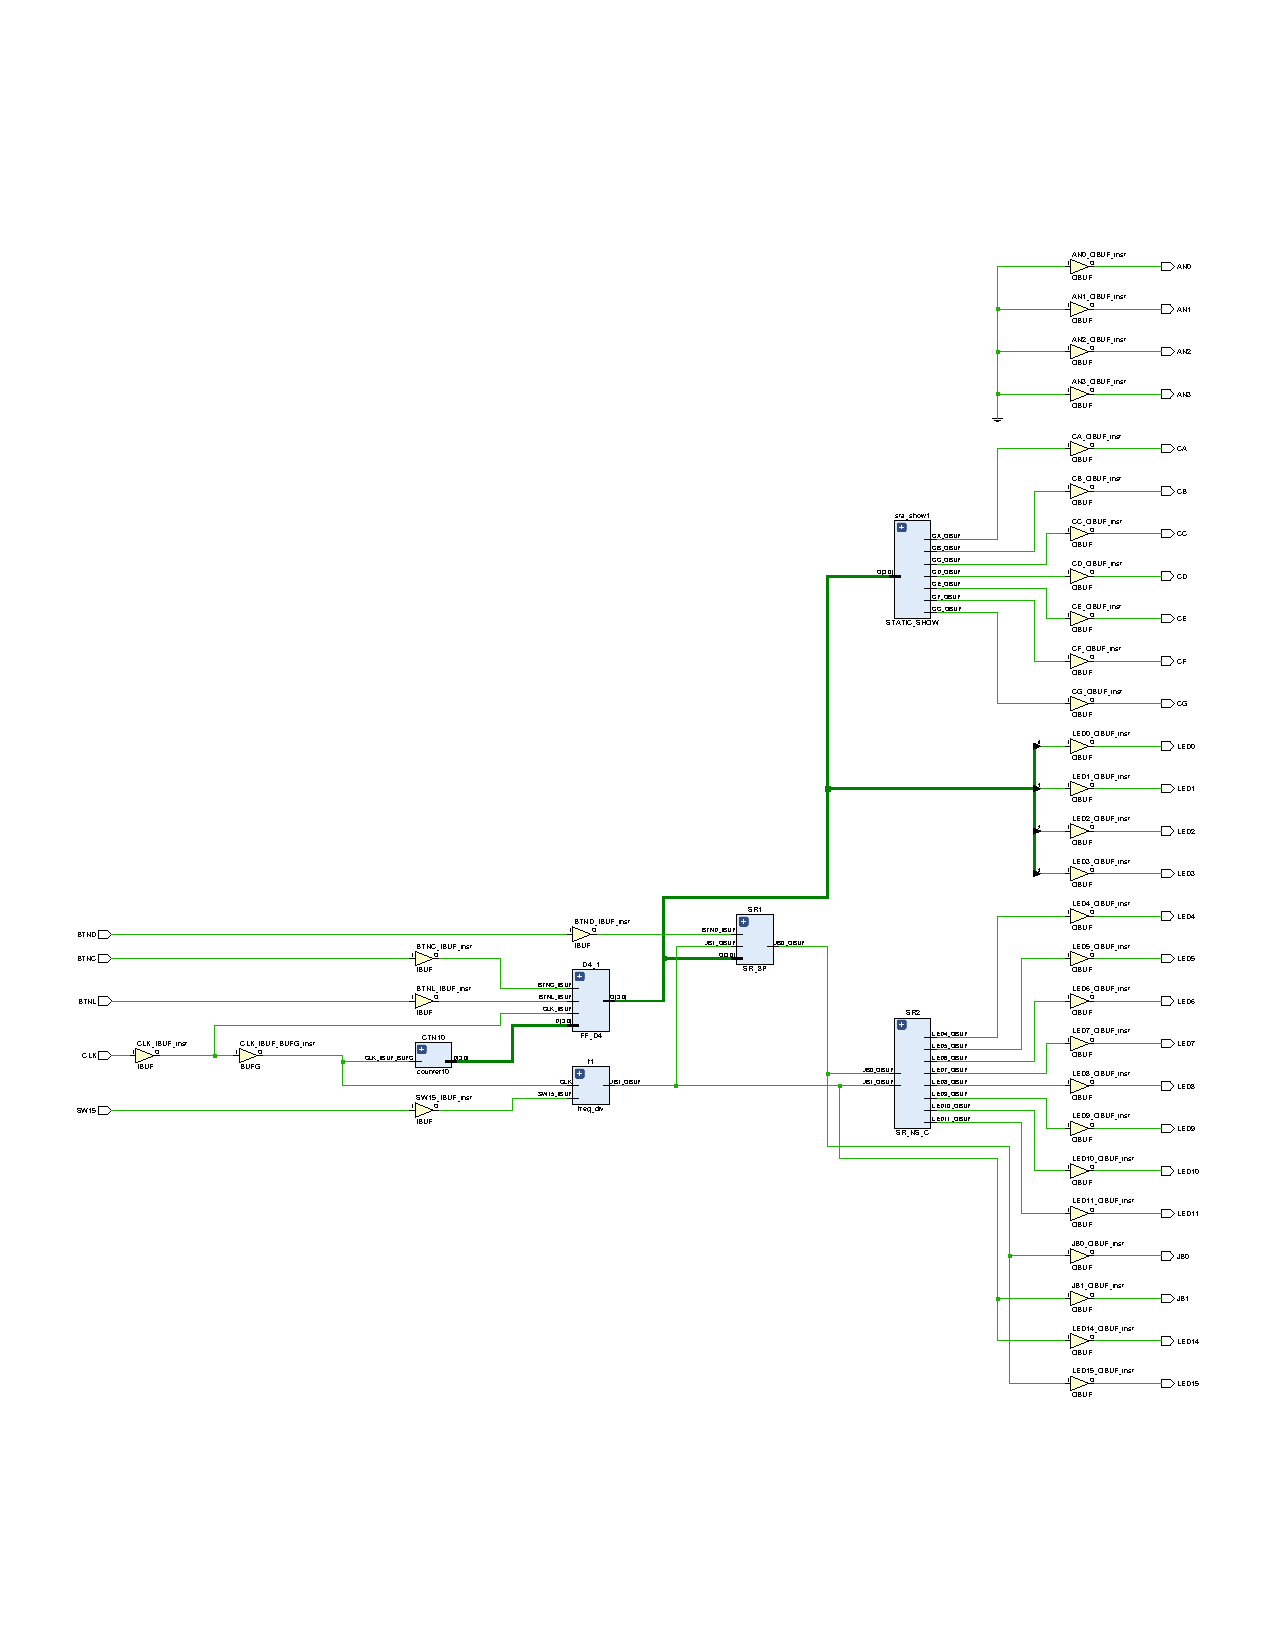
\includegraphics[width=0.8\textwidth]{pics/DataSR/sender schematic.pdf}
    \end{center}
    \caption{发送端Vivado综合电路}
    \label{send synth circuit}
\end{figure}

\begin{figure}[H]
    \begin{center}
        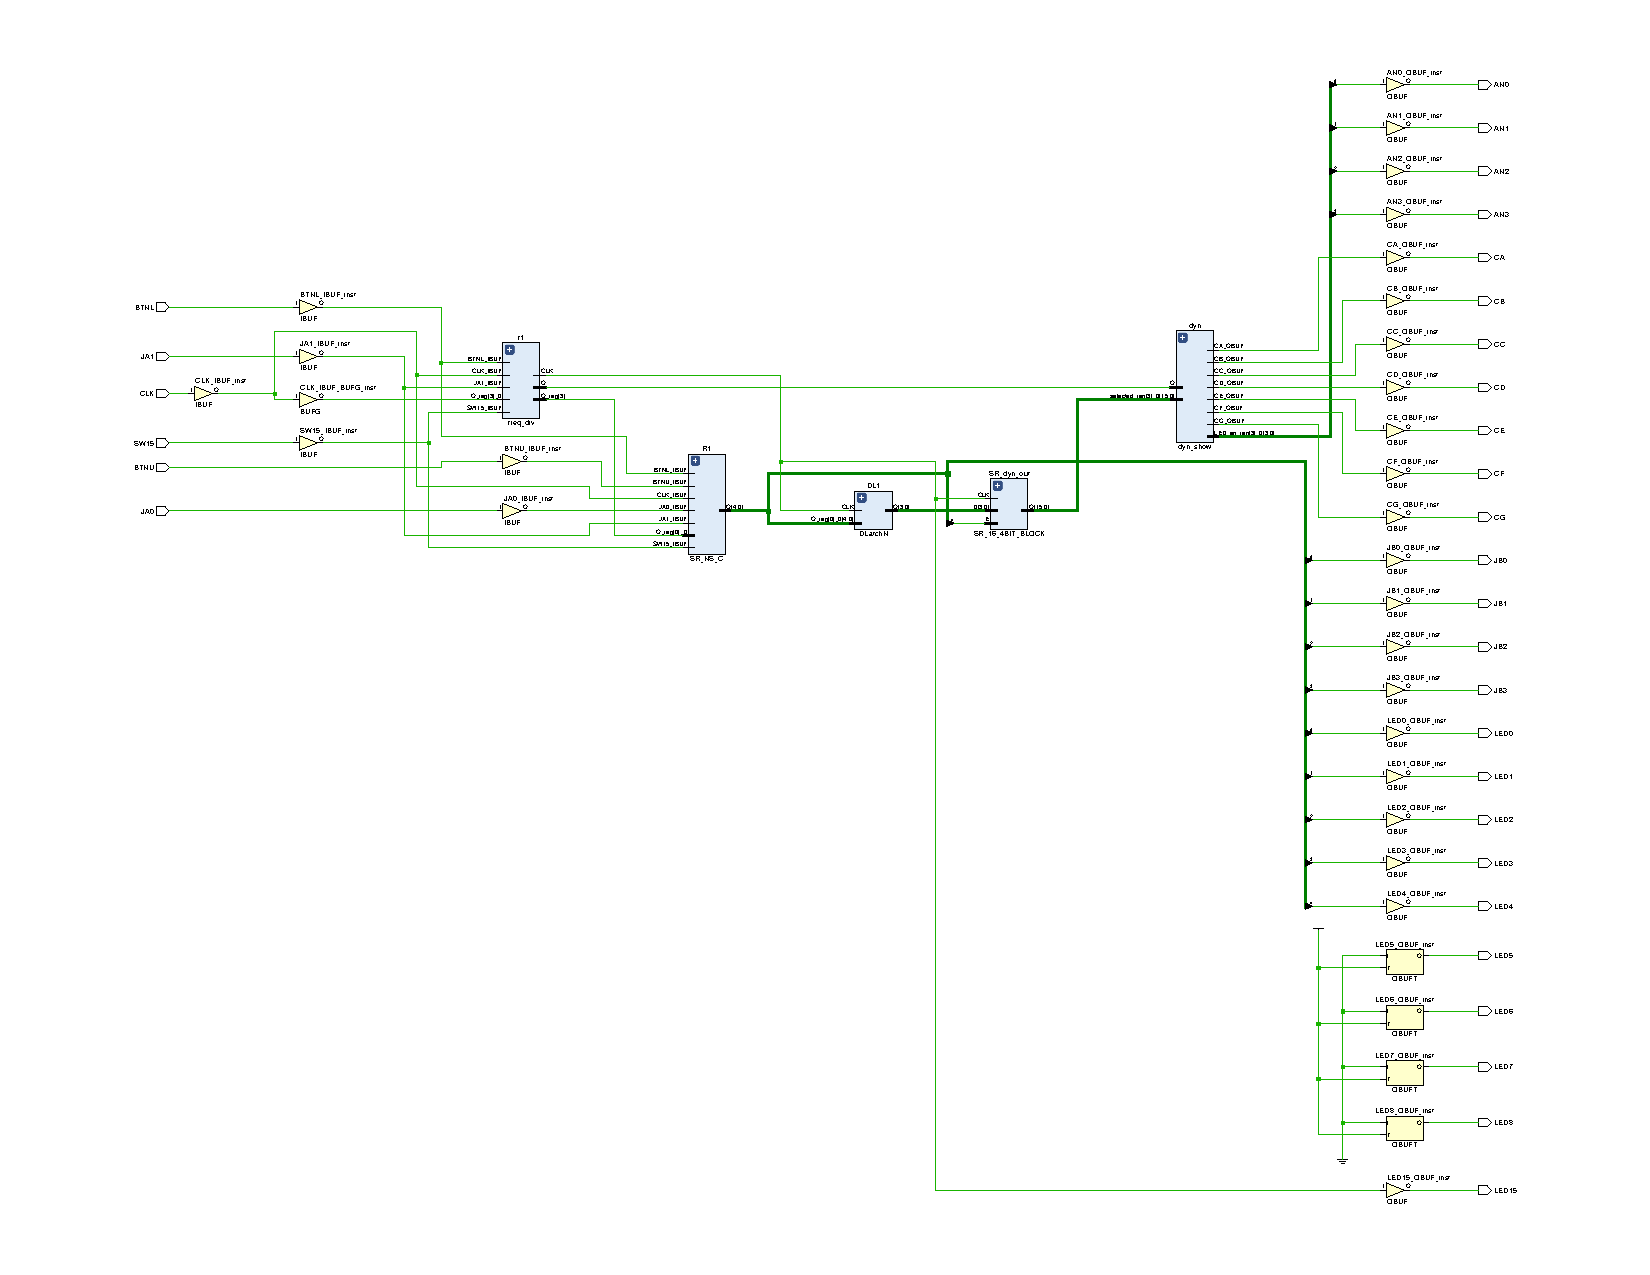
\includegraphics[width=0.8\textwidth]{pics/DataSR/receiver schematic.pdf}
    \end{center}
    \caption{接收端Vivado综合电路}
    \label{receiver synth circuit}
\end{figure}

\par 下载到开发板,观察实验现象,可以看到从发送端发送的数据可以被接收端正常接收,如图\ref{dataSR exp}所示。可以看到,先接收到的数据再后续数据到达后被移位至BCD高位显示,实现了预定功能。

\begin{figure}[H]
    \centering
    \subfigure[输入6、0]{
    \includegraphics[width=0.45\textwidth]{pics/DataSR/1.jpg}}
    \subfigure[继续输入0、9]{
    \includegraphics[width=0.45\textwidth]{pics/DataSR/2.jpg}}
    \caption{数据收发器-实际测试}
    \label{dataSR exp}
\end{figure}


\section{实验总结}
\begin{enumerate}
    \item 了解了移位寄存器工作原理,验证了移位寄存器功能
    \item 验证了JK触发器的工作状态以及相应功能
    \item 利用移位寄存器,结合verilog以及vivado实现了数据收发器
\end{enumerate}

\section*{原始数据}
\includepdf[pages=1-2]{Data_SR/dataSR preview}
\includepdf[pages=1-5]{assets/exp_data.pdf}


\end{document}